\label{proposed_system}

\subsection{Hệ thống đề xuất}

\begin{figure}[b!]
    \centering
    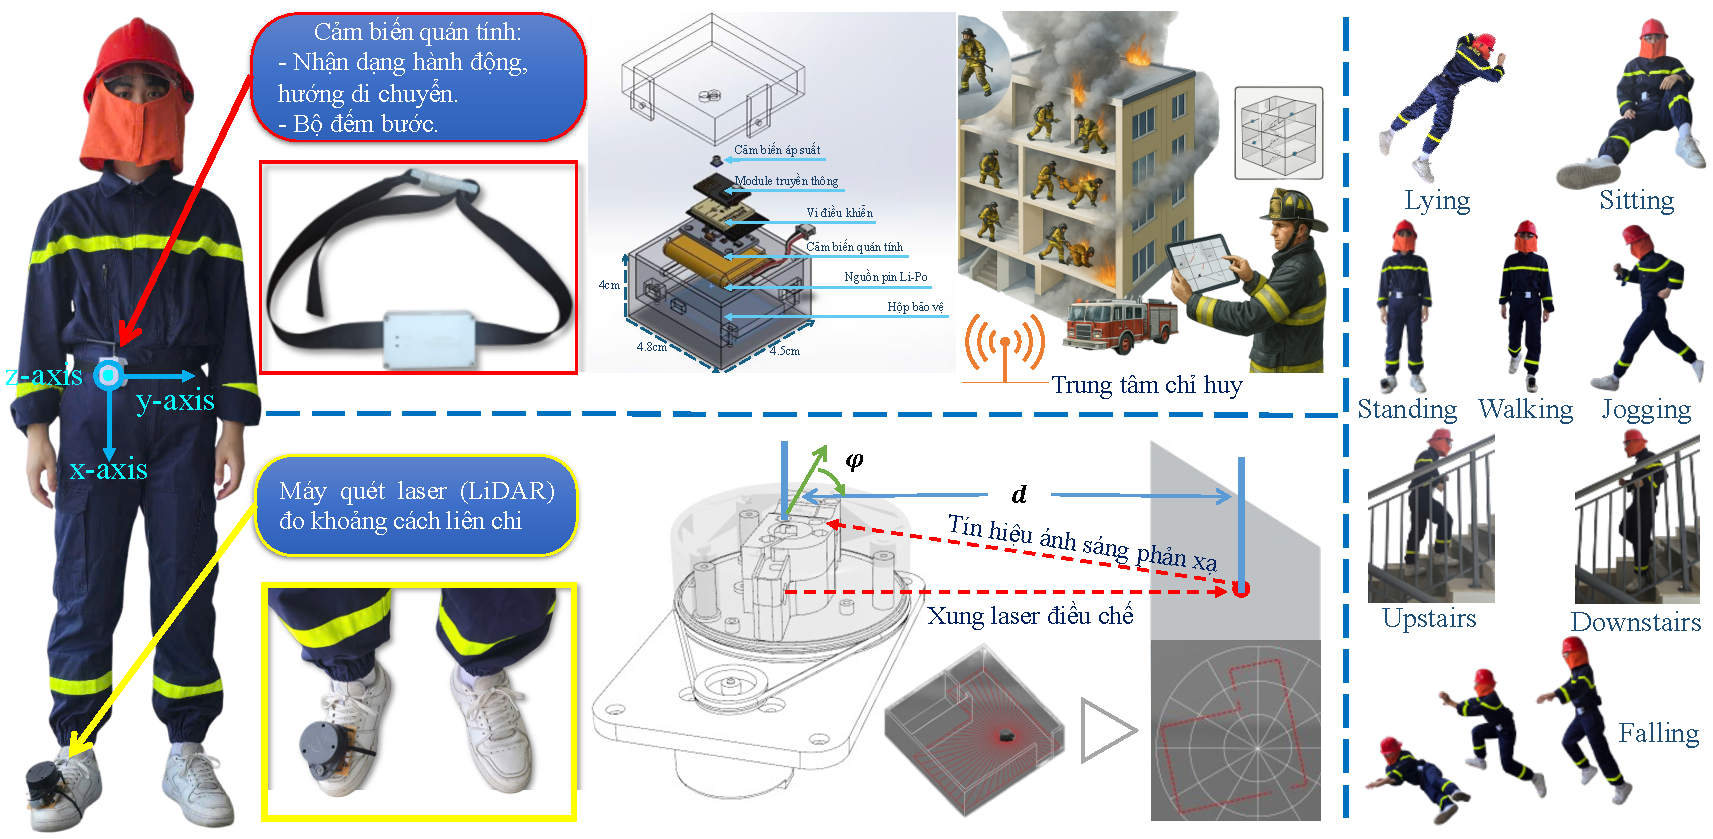
\includegraphics[width=1\linewidth]{Figure/graphical_abstract.pdf}
    \caption{Tổng quan hệ thống}
    \label{graphical_abstract}
\end{figure}

Trong nghiên cứu này, nhóm nghiên cứu phát triển một hệ thống định vị tích hợp gồm IMU 6 trục GY-85 (bao gồm gia tốc kế ADXL345 và con quay hồi chuyển ITG3200), khí áp kế GY-37, máy quét phạm vi laser RPLIDAR A1M8 và module truyền thông không dây nRF24L01, được điều khiển bởi vi điều khiển ESP-32U có hiệu suất trung bình (Hình~\ref{graphical_abstract}). Hệ thống IMU có thiết kế nhỏ gọn với kích thước 4,8 $\times$ 4,5 $\times$ 4~$\text{cm}^3$, được bố trí tại vùng eo nhằm thu thập dữ liệu chuyển động của cơ thể trong các trạng thái vận động khác nhau. Nguồn năng lượng cho hệ thống được cung cấp bởi pin Lithium-Ion Polymer 3,7~V - 600~mAh.

Để đảm bảo tính di động và ổn định, máy quét laser 2D 360° RPLIDAR A1M8 từ SLAMTEC đã được lựa chọn nhờ chi phí thấp và khả năng quét toàn diện trong phạm vi lên đến 12~m với bước sóng laser 795~nm. Thiết bị này hoạt động dựa trên nguyên lý đo tam giác, cung cấp dữ liệu đám mây điểm 2D có thể được sử dụng để lập bản đồ, định vị và mô hình hóa đối tượng/môi trường. Trong nghiên cứu này, RPLIDAR A1M8 được gắn tại mu bàn chân phải, phát tia laser đến bàn chân trái và đo thời gian phản xạ để tính toán khoảng cách chính xác. Thiết bị có khả năng hoạt động ổn định cả trong nhà lẫn ngoài trời, không bị ảnh hưởng bởi ánh sáng mặt trời trực tiếp.

Hệ thống IMU và LiDAR thu thập dữ liệu đồng thời với tần số lấy mẫu 100~Hz. Tần số này đảm bảo ghi nhận đầy đủ các chi tiết chuyển động mà không làm tăng đáng kể chi phí tính toán trên MCU. Cấu trúc dữ liệu thu thập bao gồm: Dấu thời gian (µs); Gia tốc 3 trục $\mathrm{a_x}$, $\mathrm{a_y}$, $\mathrm{a_z}$ ($\mathrm{g} =$ 9,8~$\mathrm{m\cdot s^{-2}}$); Vận tốc góc 3 trục $\mathrm{g_x}$, $\mathrm{g_y}$, $\mathrm{g_z}$~($\mathrm{rad/s}$); Khoảng cách~($\mathrm{mm}$); Góc quét~($\mathrm{degree}$); và Áp suất khí quyển~($\mathrm{mbar}$).

\begin{figure}[t]
    \centering
    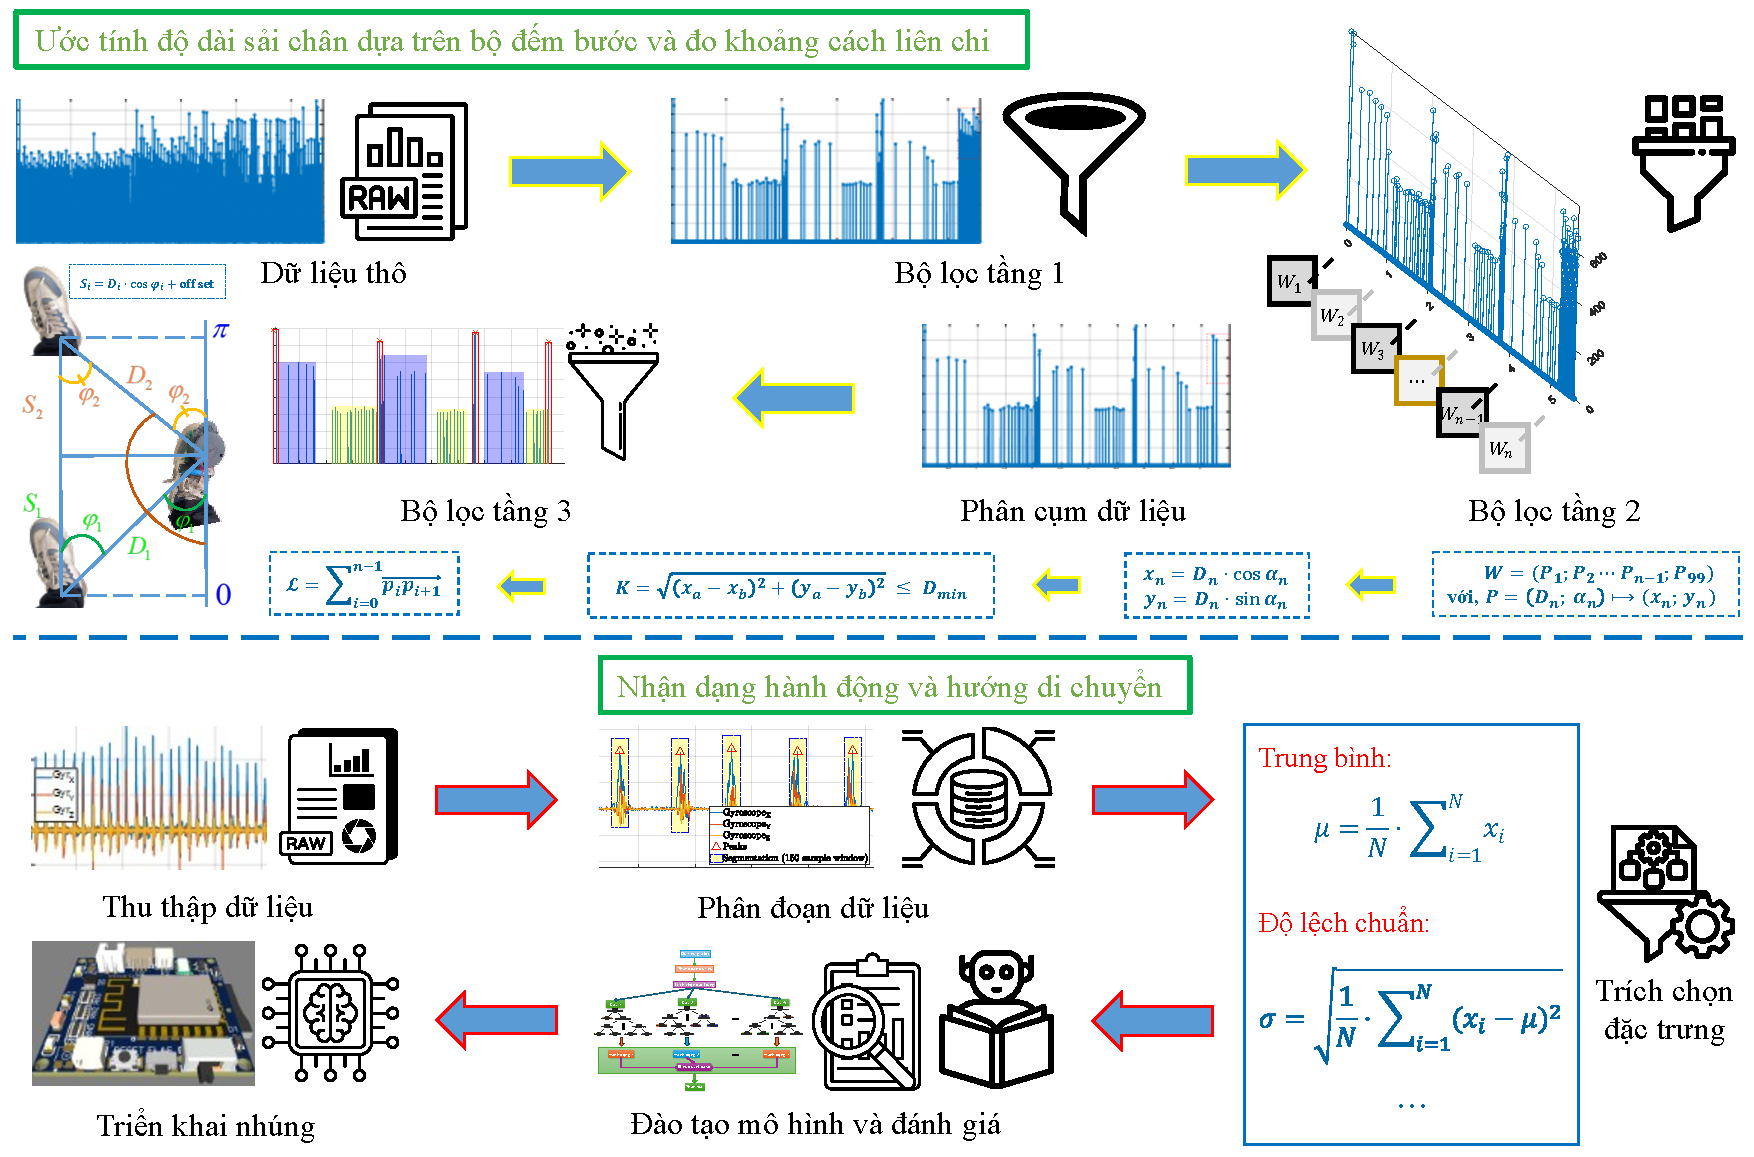
\includegraphics[width=1\linewidth]{Figure/overview_method.pdf}
    \caption{Tổng quan phương pháp phân tích dữ liệu}
    \label{overview_method}
\end{figure}

Phương pháp phân tích dữ liệu của hệ thống được minh họa trong (Hình~\ref{overview_method}). Cụ thể, gia tốc kế đảm nhận vai trò nhận dạng hành động và đếm bước, trong khi con quay hồi chuyển được sử dụng để xác định hướng di chuyển. LiDAR chịu trách nhiệm đo khoảng cách và góc quét. Trung tâm xử lý dữ liệu là vi điều khiển ESP-32U, có nhiệm vụ tiếp nhận và xử lý dữ liệu từ các cảm biến, sau đó chuyển đổi dữ liệu về hệ quy chiếu chuyển động để tính toán quãng đường và hướng di chuyển.

Để truyền dữ liệu không dây, hệ thống sử dụng hai module nRF24L01 hoạt động ở tần số 2,4~GHz. Tại trạm chỉ huy, dữ liệu được truyền đến Raspberry Pi 4 và lưu trữ vào cơ sở dữ liệu MySQL. Từ đây, dữ liệu được xử lý và hiển thị lên giao diện người dùng thông qua giao thức HTTP, cho phép truy xuất thông tin từ các thiết bị như máy tính cá nhân, laptop hoặc máy tính bảng.

Các thông tin quan trọng về tình trạng của nhân viên cứu hộ như dấu hiệu sinh tồn (giám sát hành động, phát hiện ngã) và vị trí (quãng đường di chuyển, hướng di chuyển) được trực quan hóa trên bản đồ tòa nhà theo thời gian thực. Điều này không chỉ giúp trạm chỉ huy theo dõi và cập nhật liên tục vị trí và tình trạng của từng nhân viên cứu hộ mà còn hỗ trợ đưa ra các quyết định kịp thời, nâng cao hiệu quả và đảm bảo an toàn trong quá trình cứu hộ.

